% Chapter 3

\chapter{Modelisation de l'EDP en 2D} % 3rd chapter title

\label{Chapter3} % For referencing the chapter elsewhere, use \ref{Chapter3} 

%----------------------------------------------------------------------------------------

Ayant resolu le modele en 1D durant le stage, on procede dans cette partie a sa modelisation en 2D. Il s'agit de resoudre le probleme direct du transfer radiatif avant de passer au probleme inverse dans la partie suivante. On rappelle breivement le modele considere avant de decrite l'implementation que utilisee.

\section{Le transfert radiatif}


On considère un rayonnement transporté par des particules de masse nulle appelés photons. Lorsqu'ils se touvent en presence de la matiere, les photons inteassgissent avec celle. Trois phonomees sont preponderant (figure \ref{fig:TransferRadiatif}):

\begin{figure}[!h]
\centering
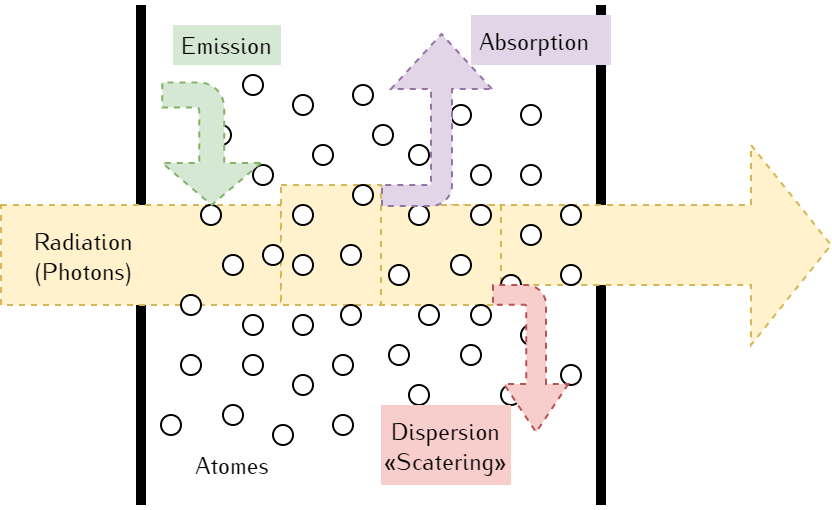
\includegraphics[width=.5\linewidth]{TransferRadiatif} 
\decoRule
\caption[TransferRadiatif]{Illustration des interaction entre radiation et matiere.}
\label{fig:TransferRadiatif}
\end{figure}

\begin{itemize}
 \item l'emission: Les photons sont emis en reponse aux electrons excites descendants a des niveaux d'energie plus bas. Ce phenomenes est caraterise par l'opacite d'émission $\sigma_e$. Il s'agit de l'inverse du libre parcours d'emision \footnote{Le libre par cours moyen d'emission represente la distance moyenne entre deux emissions de photons. Les libres parcours d'absorption et de dispersion sont definis de maniere similaire}. Plus la temperature matiere est elevee, plus ce phenomene est important.
 \item l'absorption: A l'inverse, certains photons sont absorbes par la matiere. Ce pehenomene se caraterise par l'opacite d'absorption $\sigma_a$. Lorsqu'on est a l'equilibre thermique, $\sigma_e = \sigma_e$.
 \item la dispersion (ou "scaterring" ou parfois diffusion): Certains photons sont devies de leur trajectoire par la matiere. Ce phenomme se caraterise non seulement par son opacite de scatering $\sigma_c$ \footnote{ $\sigma_a$ et $\sigma_c$ sont definis de maniere similaire a $\sigma_e$}, mais aussi par une fonction de distribution angulaire decrivant la maniere dont les photons sont devies.
\end{itemize}

L'equation du transfer radiatif (ETR) (equation \ref{eqn:ETR}) represente un bilan d'energie lie au rayonnement au niveau microscopique. Nous nous placerons dans le cas particulier d'equilibre thermodynamique local (ETL)\footnote{etat dans lequel on peut definir une temperature pour chaque point du domaine, et l'emission est decrite par la fonction de Planck \parencite{Reference3}}. L'equilibre radiatif \footnote{il se produit si la matiere est a l'equilibre avec le reyonnement. Si on est dans l'ETL, les photons sont emis suivant la fonction de Planck a la temperature de la matiere} quant a lui sera considere comme condition initiale pour les simulations.
\begingroup
\footnotesize
\begin{gather}
    \begin{aligned}
    \frac{1}{c} \frac{\partial}{\partial t}I(t,\bvec{x},\bm{\Omega},\nu)+\bm{\Omega}\cdot\nabla_x I(t,\bvec{x},\bm{\Omega},\nu)
    &= \sigma_a(\rho,\bm{\Omega},\nu)\left(B(\nu,T)-I(t,\bvec{x},\bm{\Omega},\nu)\right) \\
    &+ \frac{1}{4\pi} \int_{0}^{\infty} \int_{S^2}\sigma_c(\rho,\bm{\Omega},\nu)p(\bm{\Omega}^\prime\rightarrow\bm{\Omega})\left(I(t,\bvec{x},\bm{\Omega}^\prime,\nu)-I(t,\bvec{x},\bm{\Omega},\nu)\right) \, d\bm{\Omega}^\prime \, d\nu
    \end{aligned}
\label{eqn:ETR}
\end{gather}
\endgroup
Ou $I$ represente l'intensite specifique de radiation et $p$ ( telle que $\oint p(\bm{\Omega}^\prime\rightarrow\bm{\Omega})\, d\bm{\Omega}^\prime=1$) est la fonction de distribution angulaire de "stareing". Les autres termes sont definis dans la tables des symboles.

Il est possible de modeliser l'ETR a travers plusieurs modeles. Le modele P1 est un modele macroscopique \footnote{ils ne prennent en compte que les varaibles d'espace et de temps et spm obtenu par integration des termes microscopique tels que I par rapport a la frequence et la direction} aux moments (d'ordre 2), lineaire et hyperbolique. Vu que l'energie du rayonnement n'est pas convervee durant sont interaction avec la matiere, il faut coupler le modele P1 avec une equation regissant l'energie de la matiere. On utilisera une equation d'energie amtiere simplifiee qui ne tient compte que des termes d'echange avec le rayonnement. Le modele P1 couple a la matiere est presente ci-bas \parencite{Reference2}:
\begingroup
\large
\begin{equation}
    \begin{cases}
     \partial_tE + c \ \operatorname {div} \bvec F = c\sigma_a\left(aT^4-E\right)\\
     \partial_t\bm{F} + c \ \nabla E = -c\sigma_c \bvec{F} \\
     \rho C_v \partial_t T = c \sigma_a \left(E-aT^4\right)
    \end{cases}
\label{eqn:P1}
\end{equation}
\endgroup
Dans l'equation \ref{eqn:P1}, $\sigma_a et \sigma_c$ sont ecris sans indiquer leurs arguemnts \footnote{juste $\rho$ et $T$ si on se place dans l'ETL} afin de faciliter les notations. $E, F, \text{et} T$ represeten trepectivement l'energie des photons, le flux de phtons, et la temperature radiative. Partant de l'equation \ref{eqn:ETR}, $E$ et $T$ sont definies de la maniere suivante:
\begin{align*}
E(t,\bvec{x}) &= \frac{4\pi}{c} \int_{0}^{\infty} \int_{S^2} I(t,\bvec{x},\bm{\Omega},\nu) \, d\bm{\Omega} \, d\nu \\
\bvec{F}(t,\bvec{x}) &= \frac{4\pi}{c} \int_{0}^{\infty} \int_{S^2} \bm{\Omega}I(t,\bvec{x},\bm{\Omega},\nu) \, d\bm{\Omega} \, d\nu 
\label{eqn:EFT}
\end{align*}

Comme on peut le voir a travers la definition de $E$ et $F$, notre modele est dit "gris" car nous l'integrons sur tout le spectre de frequence. En effet, nous ne nous interressons qu'au rayonnement a travers son bilan d'energie transporte par le flux radiatif. Sur ce point, la version du modele P1 que nous avons utilise est mois precise qu'un modele microscopique base soit sur une methode Monte-Carlo ou une methode des ordonnes discrete. Neanmoins notre modele presente l'avantage d'etre tres peu couteux et relativement facile a implementer \parencite{Reference3}. 

%----------------------------------------------------------------------------------------

\section{Schéma de splitting}

Le modele P1 tend vers une equation de diffusion lorsque les opcites d'absorption ($sigma_a$) et de dispersion ($sigma_c$) sont elevees (de facon a ce que $c/sigma_a = 1$). Les schema classiques tels que le schema de Rusanov ne sont pas assez precis pour capturer cette propriete \parencite{Reference4}. 
\begin{equation}
\partial_t \left( aT^4 + \rho C_v T \right) - \operatorname{div} \left(\frac{acT^3}{\sigma_a} \nabla T \right) = O\left( \frac{1}{c} \right)
\end{equation}
Le schema en 2 etape (ou de Splitting) propose par (franck) est assez precis pour traduire la limite de diffusion. Les deux etapes sont resumees co-bas.


\subsection{Etape 1}
La premiere etape (dite etape de couplage ou d'equilibre, ou etape de relaxation de la temperature) permet de regler la temperature sur chaque maille (independament des autres mailles). On ne considere que les equations ou la temperature est impiquee (equations 1 et 3 du modele P1 \ref{eqn:P1}), en fixant la valeur du flux sur chaque maille. Il s'agit d'une methode de point fixe qui est toujorus definie. \parencite{Reference2}

Le domaine rectangulaire est suppose discretise en $N \times M$ mailles uniformes. On se trouve sur la maille $j$ (Figure \ref{fig:2DMesh}) a l'etape d'iteration $n$.

On pose donc $\Theta = aT^4$ et on obtient lw syteme:
\begingroup
\normalsize
\begin{equation*}
    \begin{dcases}
     \dfrac{E_j^{q+1} - E_j^{n}}{\Delta t} = c \sigma_a ( \Theta_j^{q+1} - E_j^{q+1}) \\
     \rho_j C_v \mu_q \dfrac{\Theta_j^{q+1} - \Theta_j^{n}}{\Delta t} = c \sigma_a (E_j^{q+1} - \Theta_j^{q+1}) 
    \end{dcases}
% \label{eqn:Step1}
\end{equation*}
\endgroup
Ou $\mu_q = \dfrac{1}{T^{3,n} + T^{n}T^{2,q} + T^{q}T^{2,n} + T^{3,q}}$.

L'etape revient a resoudre un systme de Cramer. On obtient au final:
\begin{equation} 
    \begin{dcases}
     E_j^{q+1} = \dfrac{\alpha E_j^n + \beta \gamma \Theta_j^n}{1 - \beta \delta} \\
     \Theta_j^{q+1} = \dfrac{\gamma \Theta_j^n + \alpha \delta E_j^n}{1 - \beta \delta} 
    \end{dcases}
\label{eqn:Step1}
\end{equation}
Avec $\quad  \alpha = \dfrac{1}{\Delta t \left( \frac{1}{\Delta t} + c \sigma_a \right)} ,\quad 
\beta = \dfrac{c \sigma_a}{\frac{1}{\Delta t} + c \sigma_a} ,\quad 
\gamma = \dfrac{\rho_j C_v \mu_q}{\Delta t \left( \frac{\rho_j C_v \mu_q}{\Delta t} + c \sigma_a \right)} \quad \text{et} \quad  
\delta = \dfrac{c \sigma_a}{\frac{\rho_j C_v \mu_q}{\Delta t} + c \sigma_a}.$

On itere ainsi sur q jusq'a ce que E et $\Theta$ convergent vers $E^*$ et $\Theta^*$. F reste inchange dutant cette etape.

\subsection{Etape 2}
Il s'agit ici de resoudre les deux EDP hyperboliques en 1 et 2. 
Avasnt d'qttquer le schema schema de splitting, on note que les equations 1 et 2 du modele P1 (equation \ref{eqn:P1}) sont hyperboliques et que La methode des volumes finis est donc adaptee pour les resoudre. On se place sur une maille j caracterisee par son volule $\Omega_j$.
\begin{equation*} 
    \begin{dcases}
    \partial_t \int_{\Omega_j} E + c \int_{\Omega_j} \operatorname{div} \bvec F  = 0\\
    \partial_t \int_{\Omega_j} \bvec{F} + c \int_{\Omega_j} \nabla E = -c \sigma_c \int_{\Omega_j} \bvec F 
    \end{dcases}   
% \label{eqn:VolFin}
\end{equation*}

On definit une normale $\bvec n_j$ a la surface $\Omega_j$ (voir figure \ref{fig:Discretisation2D} B) et on applique le theoreme de la divergence. On moyenne les integrales sur chaque mailles pour obtenir:
\begin{equation} 
    \begin{dcases}
    \partial_t E_j + \frac{c}{\left|\Omega_j\right|} \int_{\partial\Omega_j} \left( \bvec F, \bvec n_j  \right) = 0\\
    \partial_t \bvec{F}_j + \frac{c}{\left|\Omega_j\right|} \int_{\partial\Omega_j} \left( E, \bvec n_j  \right)= \frac{c \sigma_c}{\left|\Omega_j\right|} \int_{\Omega_j} \bvec F
    \end{dcases}   
\label{eqn:VolFin}
\end{equation}
Avec $$ E_j(t) = \frac{1}{\left|\Omega_j\right|} \int_{\Omega_j} E(t,\bvec x) \quad \text{et} \quad \bvec F_j(t) = \frac{1}{\left|\Omega_j\right|} \int_{\Omega_j} \bvec F(t,\bvec x) $$
Nous retournons donc sur le maillage disretise en definisant les different flux numeriques impliques. Durant cette etape, il faut considerer l'ajout de mailles fantommes, ce qui porte le nombre total de volumes a $(N+2) \times (M+2)$.

\begin{figure}[H]
\begin{subfigure}{.6\textwidth}
  \centering
  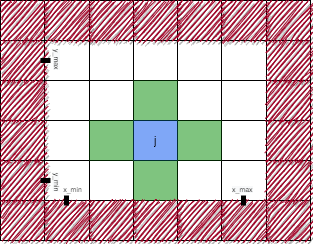
\includegraphics[width=.8\linewidth]{Dicretisation2D}  
  \caption{Dicretisation du domaine}
  \label{fig:Discretisation2D}
\end{subfigure}
\begin{subfigure}{.4\textwidth}
  \centering
  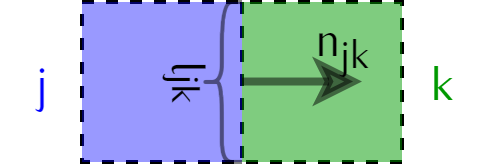
\includegraphics[width=.8\linewidth]{Interaction2D}  
  \caption{Interaction entre deux mailles j et k}
  \label{fig:Interaction2D}
\end{subfigure}

\centering
\decoRule
\caption{Dicretisation du maillage 2D. Sur la figure (A), on peut observer les mailles dites "fantomes" hachurees en rouge. Les quatre maille voisine d'une maille j sont indiquees en vert. Le volume de la maille j est definie par $\Omega_j$. Le nombre de mailles suivant l'rizontale $M$ est choisi telle que le maillage soir uniforme i.e $\Delta x = \frac{x_{max}-x_{min}}{N} = \frac{y_{max}-y_{min}}{M} = \Delta y$. Sur la figure (B), on observe la defintion de la normale sortante $n_{jk}$ de la mailles j. On peut aussi observer la longeur caracteristique $l_{jk}$}
\label{fig:2DMesh}
\end{figure}

Les flux numeriques a l'etape d'iteration $n$ sont definit entre une maille $j$ et sa maille voisine $k$ comme suit \parencite{Reference4}:
\begin{align*}
 \left(\bvec F_{jk}, \bvec n_{jk} \right) &= l_{jk} M_{jk} \left( \frac{\bvec F_j^n \cdot \bvec n_{jk} + \bvec F_k^n \cdot \bvec n_{jk}}{2} - \frac{E_k^n - E_j^n}{2} \right) \\
 \left( E_{jk}, \bvec n_{jk} \right) &= l_{jk} M_{jk} \left( \frac{E_j^n + E_k^n}{2} - \frac{\bvec F_k^n \cdot \bvec n_{jk} - \bvec F_j^n \cdot \bvec n_{jk}}{2} \right) \bvec n_{jk} \\
\end{align*}
En posant:
\begin{align*}
 \bvec S_j &= - \left( \sum_k M_{jk} \sigma_{jk} \right) \bvec F_{j}^{n+1} \\
 \bvec S_j^{\prime} &= \frac{1}{\left| \Omega_j \right|} \left( \sum_k l_{jk} M_{jk} \bvec n_{jk} \right) E_j^n \\
 M_{jk} &= \frac{2}{2 + \Delta x \sigma_{jk}}  \\
 \sigma_{jk} &= \frac{1}{2} \left( \sigma_c(\rho_j,T_j^n) + \sigma_c(\rho_k,T_k^n) \right)
\end{align*}
On peut donc ecrire cette etape du schema sous la forme:
\begin{equation*} 
    \begin{dcases}
    \frac{E_j^{n+1} - E_j^*}{\Delta t} + \frac{c}{\left| \Omega_j \right|} \sum_k \left( \bvec F_{jk}, \bvec n_{jk} \right) = 0 \\
    \frac{\bvec F_j^{n+1} - \bvec F_j^*}{\Delta t} + \frac{c}{\left| \Omega_j \right|} \sum_k \left( E_{jk}, \bvec n_{jk} \right) -c \bvec S_j^{\prime} = c \bvec{S}_j 
    \end{dcases}   
\end{equation*}
Qui se reecrit comme suit:
\begingroup
\Large
\begin{equation} 
    \begin{dcases}
    E_j^{n+1} = E_j^* + \alpha \sum_k \left( \bvec F_{jk}, \bvec n_{jk} \right) \\
    \bvec F_j^{n+1} = \beta \bvec F_j^* + \bm{\gamma} E_j^n + \delta \sum_k \left( E_{jk}, \bvec n_{jk} \right)
    \end{dcases}   
\label{eqn:Step2}
\end{equation}
\endgroup
Avec 
\begin{gather*} 
\alpha = -\frac{c \Delta t}{\left| \Omega_j \right|}, \quad 
\beta = \frac{1}{\Delta t} \left( \frac{1}{\Delta t} + c \sum_k M_{jk} \sigma_{jk} \right)^{-1}, \quad 
\bm{\gamma} = \frac{c}{\left| \Omega_j \right|} \left( \frac{1}{\Delta t} + c \sum_k M_{jk} \sigma_{jk} \right)^{-1} \left( \sum_k l_{jk} M_{jk} \bvec n_{jk} \right) \\
\text{et} \delta = -\frac{c}{\left| \Omega_j \right|} \left( \frac{1}{\Delta t} + c \sum_k M_{jk} \sigma_{jk} \right)^{-1}
\end{gather*}

La condition de CFL $\Delta t < \dfrac{\Delta x}{c}$ est necessaite pour assurer la stabilite du shema. Lors de l'implementation en C++, on remarquera qu'en pratique, il faut prendre $\Delta t < 0.5 \times \dfrac{\Delta x}{c}.$ 
%----------------------------------------------------------------------------------------

\section{Implementation en C++}

Le dode de calcul 2D a ete develope durant la 5 eme semaine du stage. Etant donne des parametre physiques et geometriques du probleme, il permet d'exporter les signaux temporels $E, F \text{et} T$ sur les quatres bords du domaine. Il permet aussi dd'exporter les signaux sur l'entierete du domaine en tout temps. Ces signaux peuvent ensuite etre visualiser sous forme d'une animation a l'aide d'un notebook construit a cet effet. L'executable pour effectuer des simulations se nomme \verb|transfer| et est disponible avec le reste du code sur le repository Github \href{https://github.com/desmond-rn/projet-inverse-2d}{projet-inverse-2d}.

\subsection{Configuration du modele}

L'executable necessite un fichier de Configuration pour s'excuter (.CFG, .TXT, etc.). Les parametres a definir sont indiques ci-dessous. Les details supplementaires sont donnes en annexe \ref{AppendixA}. La meniere dont un fichier de configuration pourrait est indiquee a la figure \ref{fig:SimuCFG}.

\begin{figure}[!h]
\centering
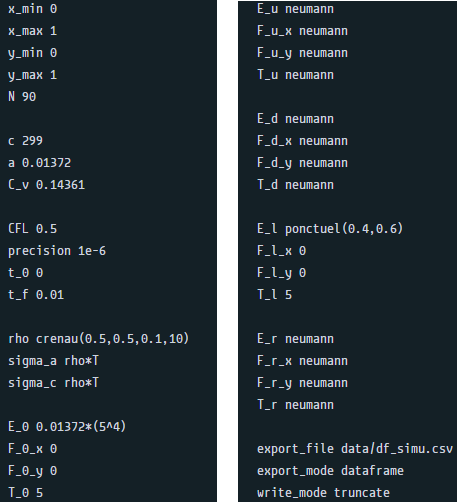
\includegraphics[width=.5\linewidth]{SimuCFG} 
\decoRule
\caption[SimuCFG]{Exemple d'un fichier de configuration au format texte. Ici ne sont representes que les 38 parametres obligatoires pour faire tourner une simualtion et l'exporter. Le resultat produit par ce fichier est presente aux figures \ref{fig:SimuCIR} et \ref{fig:EvolCIR}}
\label{fig:SimuCFG}
\end{figure}


\subsection{Sauvegarde des données}

Comme mentione ci-haut, on dispose de deux options pour sauvegarder les resultats de la simulation:

\begin{itemize}
 \item sous le forme CSV: Ce mode permet une visualisation facile des resultats a l'aide du noteook. Il est tres couteux en espace memoire et necessite la Librairie Pandas pour le lire en forme de dataframe. Cette operation prend une quantite non negligeagle de RAM, ce qui peut nuire a l'usage qu'on veut faire des donnes.
 
 \item sous le format SDS \footnote{source-densite-signal}: Ce format binaire ne sauvegarde que les informations les plus importante de la simualtion. En locurence la source utilisee, la densite du domaine, et les diffetents signaux sur les bords du domaine. Il est particulieremtnt interressant pour generer les donnees necessaires a l'apprentissage. Les details concernatn la ce format sont donnes en annexe \ref{AppendixA}.
\end{itemize}

%----------------------------------------------------------------------------------------

\section{Résultats}

Queslques resultats obtenus sont presentes ici. Les images ci-bas sont obtenus avec le fichier de configuration (IMAGE DF SIMU). La source est une onde sinusoidale placee en $E$ sur la gauche. La densitee en particulier a la forme d'un signal en crenau egale a 10 sur le crenau et 0.1 en dehors. Les opacites d'absorbes sont proportionelles a la densite.

\begin{figure}[!h]
\centering
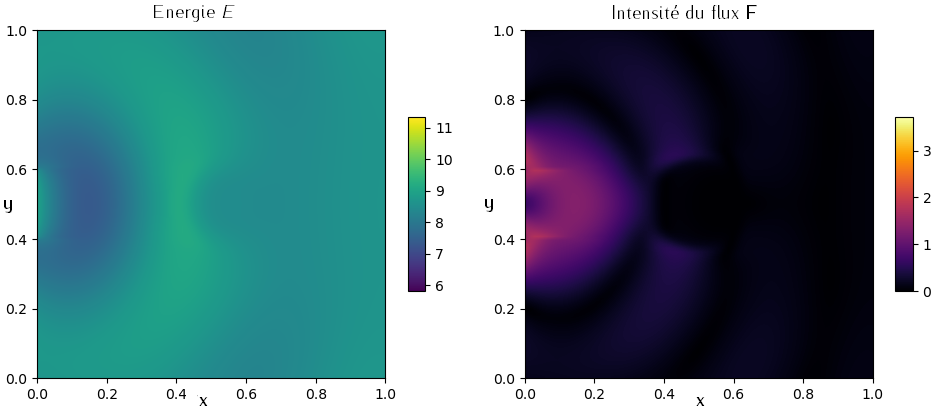
\includegraphics[width=.7\linewidth]{SimuCIR} 
\decoRule
\caption[SimuCIR]{Visualisation de l'energie et de l'intesite du flux des photons au temps final pour un domaine avec une densite en forme de crenau circulaire ((vu du haut)). Cette figure correspond aux resultat obtenus avec la simulation \ref{fig:SimuCFG}}
\label{fig:SimuCIR}
\end{figure}

La figures \ref{fig:SimuCIR} permet d'observer une asorption presque totale du signal au niveau du crenau du a la forte valeur des opacite d'absorption et de dispersion. En ce sens, le saut de densite agit comme un obstacle a la propagation du signal. l'evolution de l'energie sur les bords  du domaine (figure \ref{fig:EvolCIR} ) traduit l'effet qu'a la densite sur la propagation du signal.

\begin{figure}[H]
\centering
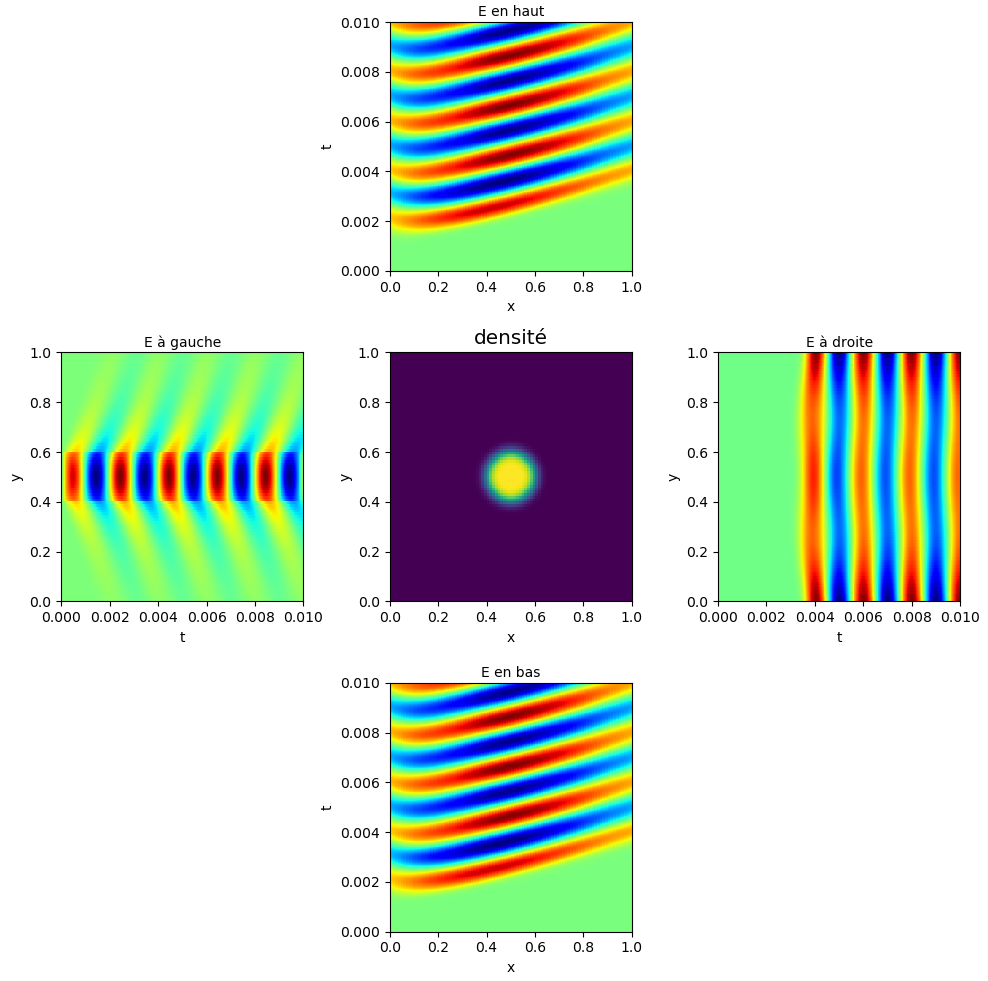
\includegraphics[width=.6\linewidth]{EvolCIR} 
\decoRule
\caption[EvolCIR]{Evolution de l'energie sur les bord (vue du haut). La cause du probleme diret (la densite) est illutree au milieu de l'image, et l'un de ses effets (E) est presntes aux alentours. Les indices x, y, et t representent repectivement l'abcisse, l'ordonne et le tempps. Les autres figures associees a ce cas sont \ref{fig:SimuCFG} et \ref{fig:SimuCIR}.  }
\label{fig:EvolCIR}
\end{figure}

Nous testons ensuite notre modele sur le cas tres particulier de l'approximation de diffusion (figures \ref{fig:SimuCFG2}, \ref{fig:SimuREC} et \ref{fig:EvolREC}) , un attout important du schema de splitting que nous avons implemente. Le bord gauche est continuement chauffe($E_{left} = a*((T_{left}+1)^4)$). La densite est un signal en forme de crenau rectangulaire (vu du haut) valant 10. En debohrs de ce crenau, la densite vaut 0.1. Theoriquement, la limite de diffusion s'observe pour$\frac{c}{\sigma_c} = 1$ (voir EQUATION ...), mais en pratique cela pose des peoblemdes de visualisation avec les coefficients que nous avons choisi. On prend donc $\sigma_a = \sigma_c = 100 \times \rho$ ce qui donne environ $\frac{c}{\sigma_c} = 30$ en dehors de l'obstacle.

On confirme effectiment l'effet de diffusion du signal dans le domaine. Nous pouvons a present passer a l'apprentissage. Pour les apprentissage, nous nous placerons essentiellement dans des conditions proches de celles de la configuration \ref{fig:SimuCFG}. Une section de l'apprentissage traitera aussi du probleme 1D non modelise ici\footnote{le probleme a ete resolu pendant le projet de CSMI}. 

\begin{figure}[!h]
\centering
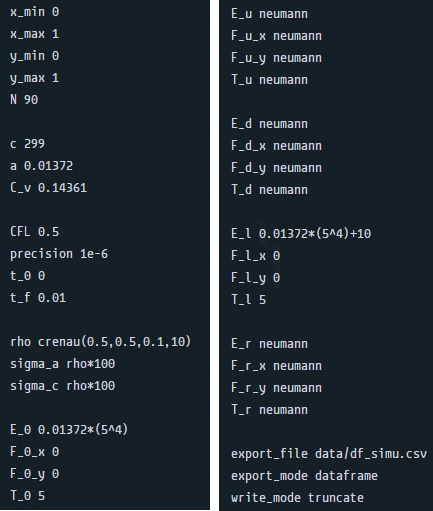
\includegraphics[width=.5\linewidth]{SimuCFG2} 
\decoRule
\caption[SimuCFG2]{Configurations utilisees pour illustrer la limite de diffusion. L'option necessaire pour obtenir un obstacle en forme de rectangule n'est pas inserable dans le fichier de configuration, cela se fait directement dans le code de calcul.}
\label{fig:SimuCFG2}
\end{figure}


\begin{figure}[!h]
\centering
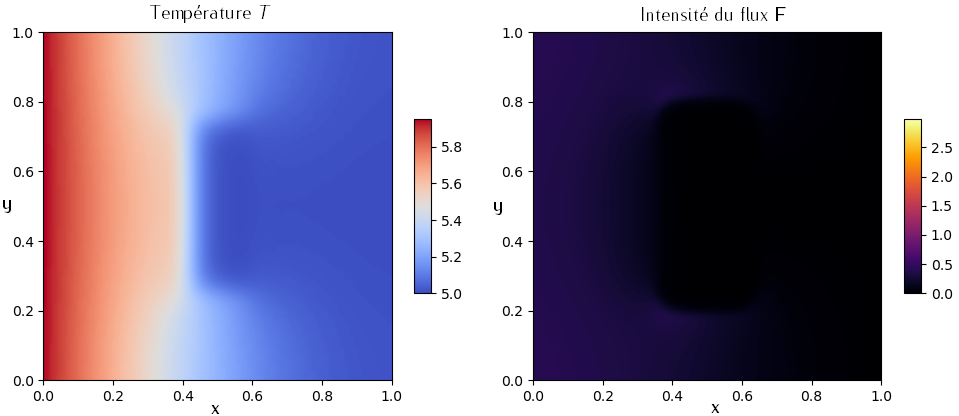
\includegraphics[width=.7\linewidth]{SimuREC} 
\decoRule
\caption[SimuREC]{Visualisation de la temperature du domaine et de l'intesite du flux des photons au temps final pour la limite de diffusion. La densite a une forme de crenau rectangulaire comme representee sur l'image du milieu de la figure \ref{fig:EvolREC}.}
\label{fig:SimuREC}
\end{figure}


\begin{figure}[!h]
\centering
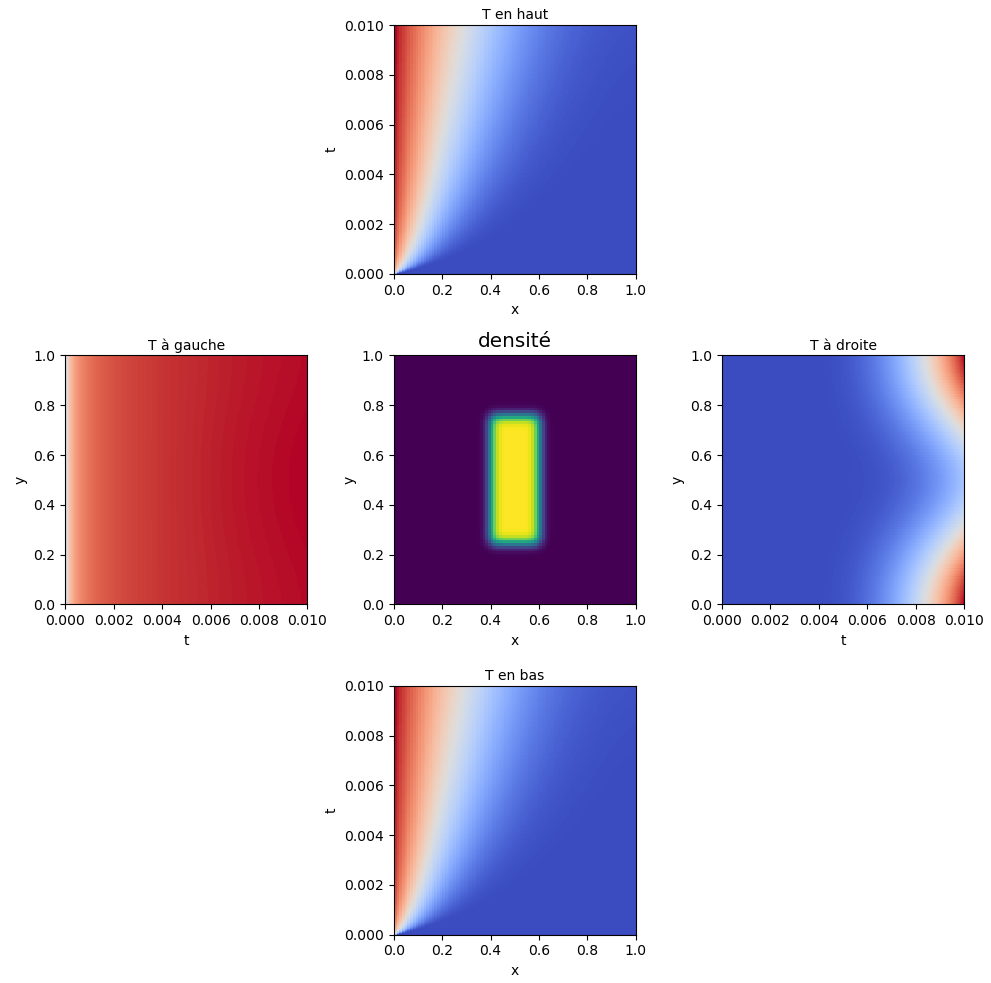
\includegraphics[width=.6\linewidth]{EvolREC} 
\decoRule
\caption[EvolREC]{Evolution de la temperature sur les bord illustrant l'effet de diffusion. Tout comme a la figure \ref{fig:SimuREC}, l'expression des opacites pour ces simulation est $\sigma_a = \sigma_c = 100 \times \rho$ afin d'obtenir un maximum de diffusion au en dehors de l'obstacle et une absorption totale sur l'obstacle.}
\label{fig:EvolREC}
\end{figure}

%----------------------------------------------------------------------------------------
